\documentclass[10pt, a4paper]{article}
\usepackage[slantfont, boldfont]{xeCJK}
\usepackage{ulem}
\usepackage{amsmath}
\usepackage{booktabs}
\usepackage{colortbl}
\usepackage[top = 1.0in, bottom = 1.0in, left = 1.0in, right = 1.0in]{geometry}
\usepackage{lipsum}
\usepackage{graphicx}
\usepackage{hyperref}
\usepackage{listings}
\usepackage{xcolor}

\usepackage{circuitikz}
% \usepackage{tikz}
% \usetikzlibrary{circuits.logic.US}


%\setCJKmainfont{SimSun}
%\setCJKmonofont{SimSun}

%\setmainfont[BoldFont={SimHei},ItalicFont={KaiTi}]{SimSun}
%\setsansfont[BoldFont=SimHei]{KaiTi}
%\setmonofont{NSimSun}

\setlength{\parskip}{0.5\baselineskip}
\setlength{\parindent}{2em}

\newcolumntype{Y}{>{\columncolor{red}}p{12pt}}
\newcolumntype{N}{>{\columncolor{white}}p{12pt}}
% \title{???}
% \author{???}


% \lstset{numbers=left,
% numberstyle=\tiny,
% keywordstyle=\color{blue!70}, commentstyle=\color{red!50!green!50!blue!50},
% frame=shadowbox,
% rulesepcolor=\color{red!20!green!20!blue!20}
% }

\lstset{
  % language=[ANSI]c,
  basicstyle=\small,
  numbers=left,
  keywordstyle=\color{blue},
  numberstyle={\tiny\color{lightgray}},
  stepnumber=1, %行号会逐行往上递增
  numbersep=5pt,
  commentstyle=\small\color{red},
  backgroundcolor=\color[rgb]{0.95,1.0,1.0},
  showspaces=false,
  showtabs=false,
  frame=shadowbox, framexleftmargin=5mm, rulesepcolor=\color{red!20!green!20!blue!20!},
% frame=single,
%  TABframe=single,
  tabsize=4,
  breaklines=tr,
  extendedchars=false %这一条命令可以解决代码跨页时,章节标题,页眉等汉字不显示的问题
}
			
\newcommand{\fullimage}[1]{
	\begin{flushleft}
		\includegraphics[width=\textwidth]{#1}
	\end{flushleft}
}
			
\newcommand{\centerimage}[1]{
	\begin{center}
		\includegraphics{#1}
	\end{center}
}

\newcommand{\pause}[0]{}


\title{Homework 2}
\author{计52 宋世虹 2015011267}
\date{2017年6月}

\begin{document}

	\maketitle

  \section{代码简介}
    我的代码有以下头文件:
      \begin{itemize}
        \item base.h: 定义了一些全局需要用的函数和变量,如eps, 点到点的距离,点到线的距离,叉乘等。
        \item Camera.h: 定义了摄像机类,摄像机存储了图像的map,并且摄像机可以发出光线来Query在某点的RGB值。
        \item Color.h:
        定义了一个点的RGB,并且重载了一些运算符。
        \item kdtree.h:
        定义了一颗KD树,用来加速K近邻查询。
        \item Light.h:
        定义了一根光线的特征。并且实现了光线的折射和反射。
        \item LightSource.h:
        定义了光源,其中有点光源和面光源,两种光源都有发射光子的功能。
        \item Object.h:
        定义了物体,包括面、盒子、球和Bezier曲面。对于每种物体都实现了求交函数,求法向量函数,和加入光子函数。
        \item Photon.h:
        定义了一个光子。
        \item PhotonMap.h:
        定义了每个物体存储光子的map,这个map可以用来计算一个点的亮度。
        \item Scene.h:
        定义了光子映射的过程,包括撒光子和渲染的过程,还有最后的保存过程。
        \item Description.txt:
        这个文件里是对于场景的描述。
      \end{itemize}
  \section{实验算法}
    \subsection{光子映射}
      具体实现:光子映射的过程是先撒光子,然后渲染场景。
      \subsection{撒光子}
        对于场景中的每一个光源,如果是点光源,就向随机方向发射光子,如果是面光源,就随机一个面上的点,把它当做点光源发射光子。发射光子的过程是,根据这个光子的方向和开始点确定一条光线,然后在Scene中使用这条光线和每个物体求交,然后这些物体和它交点离它最近的那个物体,并且在这个物体上记下这个光子,同时修改这个光子的信息,如本身的RGB,hit到物体上时光子的方向等等,用于之后渲染计算光强用。如果遇到折射和反射的情况,首先调用Light.h中的函数来计算光子下一步的方向,然后继续求交,注意这个时候会带上原物体的颜色。撒光子直到光子全部撒完为止。
      \subsection{渲染}
        渲染前先使用kdtree对撒了的光子建图,建图后就可以快速查找k近邻。对于Camera上的每个pixel渲染,都是使用和撒光子类似的方法,从相机发出一条光线,然后求交,返回交点的颜色。交点颜色的计算利用的是周围k个光子的光亮度乘以他们的颜色除以包围他们最小的球半径的平方乘以$\pi$。由于这里直接使用这样的光亮度,会使得很多东西都暗的看不清楚或者白茫茫的一片,所以我对所有的光亮度先normalize了一遍,然后乘了一个很小的系数开方,这会使图片的效果好很多。
      \subsection{扩展}
        \subsubsection{Bezier高次曲面求交}
          这里我使用的是牛顿迭代法。首先先用包围盒判断是否不相交,这个会加速很多。然后对于每条可能相交的光线,将t,u,v初始化为任意0,1之间的数,进行迭代20轮,如果不收敛重新初始化,这里有5次重新初始化机会,如果还是不能相交则为不相交,否则即为相交。

          实验中实现了25个控制点的Bezier曲面求交。

          代码段:(在Object.cpp里)
          \begin{lstlisting}
bool Bezier::isInbox(Light& light)
{
  // printf("%f %f %f\n",BoundingLB[0],BoundingLB[1],BoundingLB[2] );
  // printf("%f %f %f\n",BoundingRT[0],BoundingRT[1],BoundingRT[2] );
  for (int i = 0;i < 3;++i)
  {
    Surface* temp = new Surface(i == 0,i == 1,i == 2,-BoundingLB[i],cv::Vec3f(0,0,0));
    Point inter = temp->intersect(light);
    // printf("inter %f %f %f \n",inter[0],inter[1],inter[2]);
    bool thisinter = true;
    for (int j = 0;j < 3;++j)
      if (i != j)
        if (inter[j] >= BoundingLB[j] || inter[j] <= BoundingRT[j])
          thisinter = false;
    if (thisinter) return true;
  }
  for (int i = 0;i < 3;++i)
  {
    Surface* temp = new Surface(i == 0,i == 1,i == 2,-BoundingRT[i],cv::Vec3f(0,0,0));
    Point inter = temp->intersect(light);
    bool thisinter = true;
    for (int j = 0;j < 3;++j)
      if (i != j)
        if (inter[j] >= BoundingLB[j] || inter[j] <= BoundingRT[j])
          thisinter = false;
    if (thisinter) return true;
  }
  return false;
}

Point Bezier::intersect(Light& light)
{
  // printf("%f %f %f\n", light.direction.x,light.direction.y,light.direction.z);
  // fflush(stdout);
  bool WillInter = isInbox(light);
  // printf("%d\n", int(WillInter));
  if (!WillInter) return BackgroundPoint;
  // printf("gg\n");
  VectorXd origin(3);
  origin[0] = origin[1] = origin[2] = 0;
  VectorXd nowPoint(3);
  bool getAns = false;
  int tot = 0;
  while (!getAns && tot < 20)
  {
    nowPoint[0] = std::rand() * 1.0/RAND_MAX;
    nowPoint[1] = std::rand() * 1.0/RAND_MAX;
    nowPoint[2] = std::rand() * 1.0/RAND_MAX;
    int count = 0;
    while (1)
    {
      origin = nowPoint;
      Matrix3d derive;
      for (int i = 0;i < 3;++i)
        for (int j = 0;j < 3;++j)
          derive(i,j) = getDerivedF(i,j,origin,light);
      // std::cout << derive << std::endl;
      Matrix3d inverse;
      bool invertible;
      double determinant;
      derive.computeInverseAndDetWithCheck(inverse,determinant,invertible);
      // std::cout << inverse << std::endl;
      if(invertible) 
      {
        VectorXd value(3);
        value[0] = light.beginPoint.x + light.direction.x * nowPoint[0];
        for (int i = 0;i <= n;++i)
          for (int j = 0;j <= m;++j)
            value[0] -= P[i][j].x * getBezier(i,n,nowPoint[1]) * getBezier(j,m,nowPoint[2]);
        value[1] = light.beginPoint.y + light.direction.y * nowPoint[0];
        for (int i = 0;i <= n;++i)
          for (int j = 0;j <= m;++j)
            value[1] -= P[i][j].y * getBezier(i,n,nowPoint[1]) * getBezier(j,m,nowPoint[2]);
        value[2] = light.beginPoint.z + light.direction.z * nowPoint[0];
        for (int i = 0;i <= n;++i)
          for (int j = 0;j <= m;++j)
            value[2] -= P[i][j].z * getBezier(i,n,nowPoint[1]) * getBezier(j,m,nowPoint[2]);
        // std::cout << value << std::endl;
        // printf("%f %f %f\n", nowPoint[0],nowPoint[1],nowPoint[2]);
        if ((pow(value[0],2) + pow(value[1],2) + pow(value[2],2)) <= eps)
        {
          getAns = true;
          break;
        }
        nowPoint = nowPoint - inverse * value;
        count++;
        if (count > 20) break;
        // printf("%f %f %f\n", nowPoint[0],nowPoint[1],nowPoint[2]);
      }
      else 
      {
        // printf("invertible\n");
        break;
      }
    }
    if (nowPoint[0] > eps && nowPoint[1] > eps && nowPoint[1] < 1 && nowPoint[2] > eps && nowPoint[2] < 1 && getAns)
      break;
    else getAns = false;
    tot++;
  }
  if (nowPoint[0] > eps && nowPoint[1] > eps && nowPoint[1] < 1 && nowPoint[2] > eps && nowPoint[2] < 1 && getAns)
  {
    // printf("%f %f %f\n", nowPoint[0],nowPoint[1],nowPoint[2]);
    return Point(light.beginPoint.x + nowPoint[0] * light.direction.x,light.beginPoint.y + nowPoint[0] * light.direction.y,light.beginPoint.z + nowPoint[0] * light.direction.z,nowPoint[1],nowPoint[2]);
  }
  else return BackgroundPoint;
}

double Bezier::getBezier(int i,int m,double u)
{
  if (i < 0) return 0;
  if (u < eps || u > 1-eps) return 0;
  return C[m][i] * pow(u,i) * pow(1-u,m-i);
}

double Bezier::getBezierDerive(int i,int m,double u)
{
  return m * (getBezier(i-1,m-1,u) - getBezier(i,m-1,u));
}

double Bezier::getDerivedF(int i,int j,VectorXd& origin,Light& light)
{
  if (j == 0)
  {
    return light.direction[i];
  }
  else if (j == 1)
  {
    double temp = 0;
    for (int p = 0;p <= n;++p)
      for (int q = 0;q <= m;++q)
        temp += P[p][q][i] * getBezierDerive(p,n,origin[1]) * getBezier(q,m,origin[2]);
    return -temp;
  }
  else 
  {
    double temp = 0;
    for (int p = 0;p <= n;++p)
      for (int q = 0;q <= m;++q)
        temp += P[p][q][i] * getBezier(p,n,origin[1]) * getBezierDerive(q,m,origin[2]);
    return -temp;
  }
}
          \end{lstlisting}
        \subsubsection{贴图/景深}
          实现了给Bezier曲面贴图和整体的景深。

          贴图:对于Bezier曲面,使用它的u,v贴图,即对于每一个交点,返回它在这个交点的某个图上的RGB。具体的做法是建立u,v到这个图的映射。

          景深:对于相机发出的光线进行重采样,如果已知焦平面的位置,那么焦平面上的物体是一定能被看清的。这样我们就可以每次要想知道一个相机像素上一点的值,我们只需要从相机先发出一条光线和焦平面相交,然后对于这个交点,再从相机周围一个圆上随机采样一些点来计算新的RGB值,对这些算出的RGB重新加权得到真实的RGB。

          贴图代码片段:(在Object.cpp中)
          \begin{lstlisting}
Color Bezier::colorAt(Point& point)
{
  int col = wangzai.cols * (1-point.u);
  int row = wangzai.rows * (1-point.v);
  if (col == wangzai.cols || col == wangzai.cols-1) col = wangzai.cols - 2;
  if (row == wangzai.rows || row == wangzai.rows-1) row = wangzai.rows - 2;
  return Color(wangzai.at<cv::Vec3b>(row,col)[0] * 1.0/256,wangzai.at<cv::Vec3b>(row,col)[1] * 1.0/256,wangzai.at<cv::Vec3b>(row,col)[2] * 1.0/256) ;
}
          \end{lstlisting}

          景深代码片段:(在Camera.cpp和Scene.cpp中)
          \begin{lstlisting}
std::vector<Light> Camera::getLight(int x,int y)
{
  bool jingshen = false;
  double fl = 2.5;
  std::vector<Light> result;
  Point direction(tan( (x - position.x -(width/2)) * fov_w / width) , tan( ((height/2)-position.y-y) * fov_h / height ),1);
  direction = direction.normz();
  direction = fl * direction;
  // printf("%f %f %f\n", direction.x, direction.y, direction.z );
  Point beginPoint = position;
  result.push_back(Light(beginPoint,direction));
  if (jingshen)
  {
    double sanfenzhipi = pi/3;
    for (int i = 0;i < 6;++i)
    {
      double x1 = 0.1 * sin(sanfenzhipi * i), x2 = 0.1 * cos(sanfenzhipi * i);
      beginPoint = Point(x1,x2,0);
      Point nowDir = direction - beginPoint;
      result.push_back(Light(beginPoint,nowDir));
    }
  }
  return result;
}
for (int i = 0;i < camera->rows;++i)
    for (int j = 0;j < camera->cols;++j)
    {
      printf("%d\r",i);
      fflush(stdout);
      std::vector<Light> lights = camera->getLight(i,j);
      double right = 1.0 / lights.size();
      camera->image[i][j] = Color(0,0,0);
      for (int k = 0;k < lights.size(); ++k)
        camera->image[i][j] += right * getPointColor(lights[k],1);
    }
          \end{lstlisting}
        \subsubsection{渲染加速}
          主要由求包围盒和kd树加速。

          包围盒针对Bezier曲线使用,即取Bezier控制点的x,y,z边界建立包围盒,对于每一条光线,先判断是否和这个包围盒相交,如果不相交则一定不会和Bezier曲面相交,否则有可能和Bezier曲面相交,则继续用牛顿迭代法寻找交点。

          kd树加速,即对于光子建立kd树,每次查找k近邻的时候可以做到约根号光子数的复杂度。代码见kdtree.h。

          包围盒代码:(见Object.cpp)

          \begin{lstlisting}
BoundingLB.x = -INT_MAX;
  BoundingLB.y = -INT_MAX;
  BoundingLB.z = -INT_MAX;
  BoundingRT.x = INT_MAX;
  BoundingRT.y = INT_MAX;
  BoundingRT.z = INT_MAX;
  for (int i = 0;i <= n;++i)
  {
    std::vector<Point > tempvec;
    P.push_back(tempvec);
    for (int j = 0;j <= m;++j)
    {
      double xx,yy,zz;
      fin >> temp;
      xx = atof(temp.c_str());
      fin >> temp;
      yy = atof(temp.c_str());
      fin >> temp;
      zz = atof(temp.c_str());
      this->P[i].push_back(Point(xx,yy,zz));
      if (xx < BoundingRT.x)
        BoundingRT.x = xx;
      if (yy < BoundingRT.y)
        BoundingRT.y = yy;
      if (zz < BoundingRT.z)
        BoundingRT.z = zz;
      if (xx > BoundingLB.x)
        BoundingLB.x = xx;
      if (yy > BoundingLB.y)
        BoundingLB.y = yy;
      if (zz > BoundingLB.z)
        BoundingLB.z = zz;
    }
  }
bool Bezier::isInbox(Light& light)
{
  // printf("%f %f %f\n",BoundingLB[0],BoundingLB[1],BoundingLB[2] );
  // printf("%f %f %f\n",BoundingRT[0],BoundingRT[1],BoundingRT[2] );
  for (int i = 0;i < 3;++i)
  {
    Surface* temp = new Surface(i == 0,i == 1,i == 2,-BoundingLB[i],cv::Vec3f(0,0,0));
    Point inter = temp->intersect(light);
    // printf("inter %f %f %f \n",inter[0],inter[1],inter[2]);
    bool thisinter = true;
    for (int j = 0;j < 3;++j)
      if (i != j)
        if (inter[j] >= BoundingLB[j] || inter[j] <= BoundingRT[j])
          thisinter = false;
    if (thisinter) return true;
  }
  for (int i = 0;i < 3;++i)
  {
    Surface* temp = new Surface(i == 0,i == 1,i == 2,-BoundingRT[i],cv::Vec3f(0,0,0));
    Point inter = temp->intersect(light);
    bool thisinter = true;
    for (int j = 0;j < 3;++j)
      if (i != j)
        if (inter[j] >= BoundingLB[j] || inter[j] <= BoundingRT[j])
          thisinter = false;
    if (thisinter) return true;
  }
  return false;
}
          \end{lstlisting}
  \section{实验效果}
    \subsection{焦散和次表面折射}
      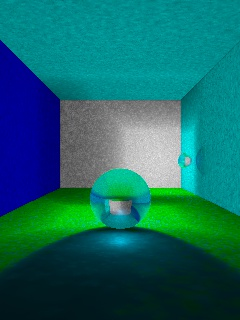
\includegraphics[scale = .6]{caustics.jpg}

      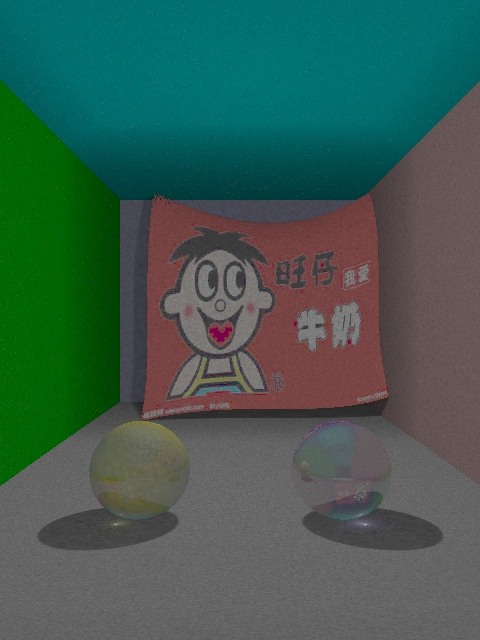
\includegraphics[scale = .6]{wangzai2.jpg}

    \subsection{贴图和景深}

      我尝试了集中景深的半径取值,后来发现取0.1好像效果比较好。贴图如图。

      半径取值0.01,几乎看不出景深:

      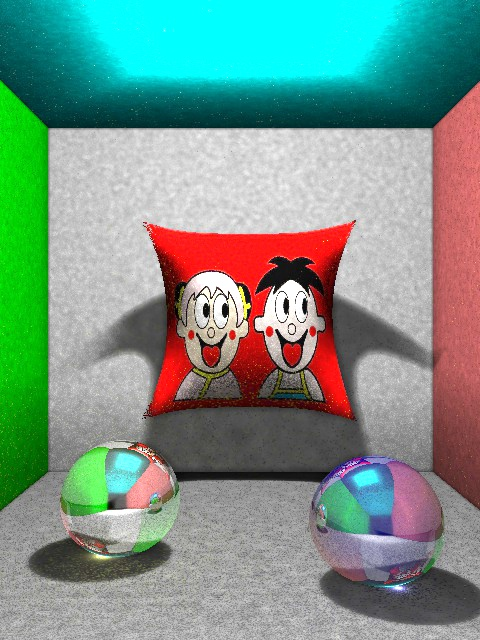
\includegraphics[scale = .6]{zhengchang3.jpg}

      半径取值0.1,效果显著:

      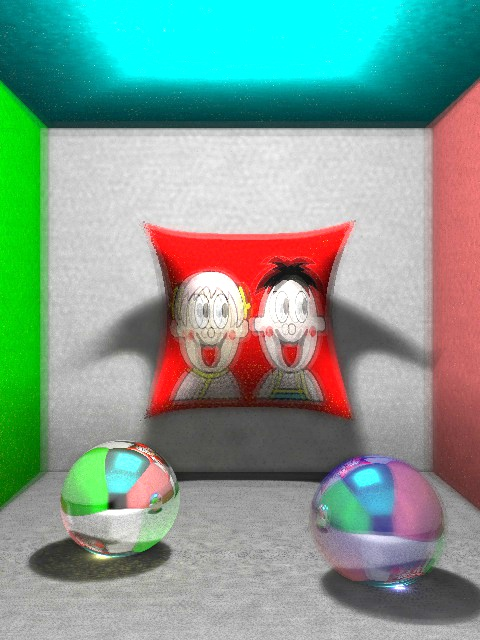
\includegraphics[scale = .6]{jingshen2F.jpg}

    \subsection{另一构景}
      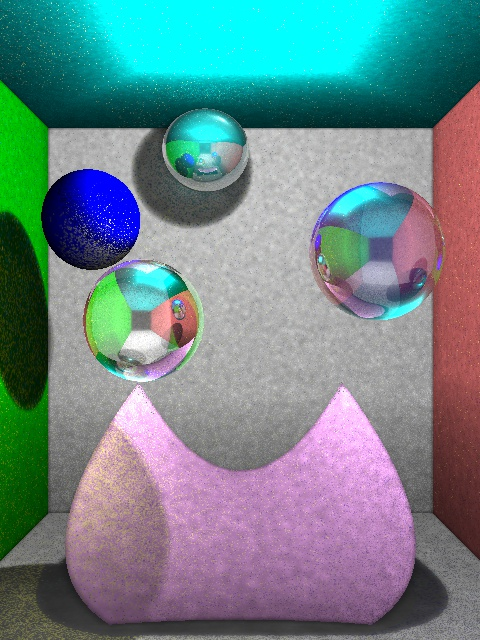
\includegraphics[scale = .6]{haokande.jpg}

\end{document}






































